\documentclass[10pt]{article}
\usepackage{titling} % Customize the title
\usepackage[utf8]{inputenc}
\usepackage{eso-pic}
\usepackage{charter}
\usepackage[margin=1in]{geometry}
\usepackage{amssymb,pdfpages,fancyhdr,subcaption,graphicx,hyperref,float,outlines,amsmath,gensymb}
\usepackage{listings}
\usepackage{parskip}
\usepackage{multicol} % Added the multicol package
\usepackage{booktabs}
\usepackage{graphicx}
\usepackage{subcaption}
\usepackage{multirow}
\usepackage{listings}
\usepackage{xcolor}

% Define colors for code highlighting
\definecolor{codegreen}{rgb}{0,0.6,0}
\definecolor{codegray}{rgb}{0.5,0.5,0.5}
\definecolor{codepurple}{rgb}{0.58,0,0.82}
\definecolor{backcolour}{rgb}{0.95,0.95,0.92}

% Define settings for Python code
\lstdefinestyle{mystyle}{
    backgroundcolor=\color{backcolour},
    commentstyle=\color{codegreen},
    keywordstyle=\color{blue},
    numberstyle=\tiny\color{codegray},
    stringstyle=\color{codepurple},
    basicstyle=\ttfamily\footnotesize,
    breakatwhitespace=false,
    breaklines=true,
    captionpos=b,
    keepspaces=true,
    numbers=left,
    numbersep=5pt,
    showspaces=false,
    showstringspaces=false,
    showtabs=false,
    tabsize=2
}

\lstset{style=mystyle}

\title{\textbf{4M17 Coursework \#2 \\ Optimisation Algorithm Performance Comparison}}
\author{\textbf{Candidate No: 5730E}}

\begin{document}
\maketitle
\section{Abstract}
This report conducts a comparative analysis of two optimisation algorithms applied to minimise Keane's Bump Function, (KBF). In particular, the study focuses on a Continuous Genetic Algorithm, (CGA), as well as an alternative algorithm not covered in the lectures: Q-learning, (QEG). Specifically, the Q-learning approach is adapted with the epsilon-greedy strategy to introduce a level of stochasticity into the optimisation process, thus aligning it with the requirements of this assignment.

\begin{figure}[H]
\centering
\begin{subfigure}{0.49\textwidth}
    \centering
    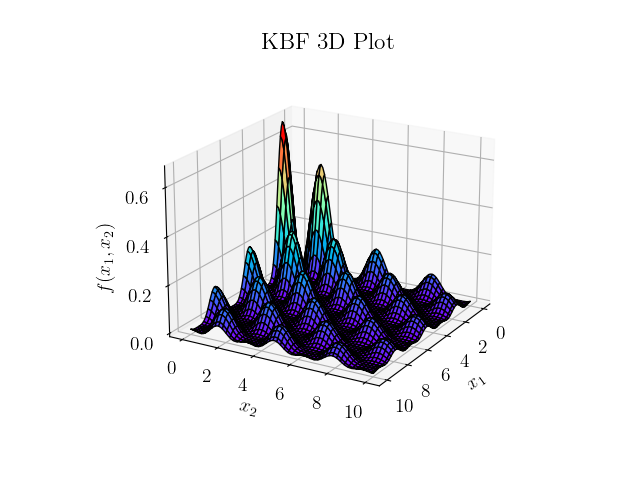
\includegraphics[width=\textwidth]{../figures/KBF/KBF_surf.png}
    \caption{Surface plot.}
    \label{fig:KBF_surf}
\end{subfigure}
\begin{subfigure}{0.49\textwidth}
    \centering
    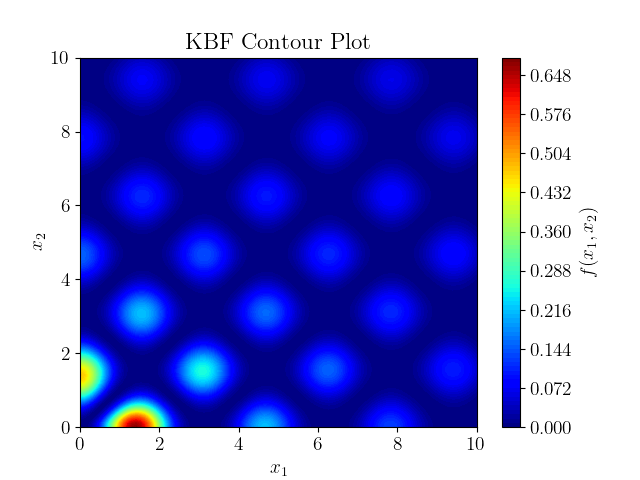
\includegraphics[width=\textwidth]{../figures/KBF/KBF_contour.png}
    \caption{Contour plot.}
    \label{fig:KBF_contour}
\end{subfigure}
    \captionsetup{justification=centering}
    \caption{The two-dimensional visualisation of the Keane's Bump Function, (KBF).}
    \label{fig:KBF_2D}
\end{figure}

\section{Introduction}
\begin{multicols}{2}
\subsection{Keane's Bump Function}
To compare the performances of the two algorithms, the Keane's Bump Function, (KBF), is used as the objective function. In particular, the n-dimensional constrained optimisation problem is defined as the maximisation of:

\begin{equation}
    f(\mathbf{x}) = \left| \frac{\sum_{i=1}^{n} (\cos(x_i))^4 - 2\prod_{i=1}^{n} (\cos(x_i))^2}{\sqrt{\sum_{i=1}^{n} i \cdot x_i^2}} \right|
    \label{eq:KBF_cost}
\end{equation}
\begin{equation}
    \begin{aligned}
        \text{subject to} \quad & 0 \leq x_i \leq 10 \quad \forall i \in \{1, \dots, n\} \\
        & \quad \prod_{i=1}^{n} x_i > 0.75 \\
        & \quad \sum_{i=1}^{n} x_i < \frac{15n}{2}
    \end{aligned} 
    \label{eq:KBF_constraints}
\end{equation}

The two-dimensional form of the function has been plotted in Figure \ref{fig:KBF_2D}. Some notable properties are as follows:

\begin{itemize}
    \item The function is undefined at the origin, (0, 0). This is due to the division by zero in the denominator of Equation \ref{eq:KBF_cost}. Otherwise, the function is continuous and differentiable everywhere.
    \item The function is highly multi-modal. Its global maximum is located on the constaint boundary $x_{n}=0$, where $x_n$ denotes the final variable in the n-dimensional space. However, there are many local maxima located inside the feasible region, all of which have quite similar amplitudes.
    \item The function is nearly symmetric about the line $x_1=x_2$. This stems from its construction in \ref{eq:KBF_cost}, using the sums of squared, symmetric terms, $x_i^2$, $(\cos(x_i))^2$, and $(\cos(x_i))^4$. This results in some invariance regarding the order of the input variables. Overall, the peaks consistently manifest in pairs, yet there is a notable pattern wherein one peak always surpasses its counterpart in magnitude.
\end{itemize}

Given the above properties, the KBF is a challenging function to optimise. The presence of multiple, similar-amplitude local maxima makes it difficult for an optimisation algorithm to converge to the global maximum. On the other hand, all control variables share the same nature, (continuous variables), and exhibit identical scales. Additionally, all constraints are of the inequality type, and the feasible space is non-disjoint.

These properties make the KBF a suitable candidate for the comparative analysis of the two optimisation algorithms, as discussed in the previous work \cite{ELBELTAGY1999639}.

\subsection{Continuous Genetic Algorithm}

The discrete nature of the GA presented in \cite{parks2023geneticalgorithms} makes it unsuitable for the optimisation of the KBF. An implementation of a Continuous Genetic Algorithm, (CGA), is used instead, which lends itself better to the problems presented in \ref{eq:KBF_cost}-\ref{eq:KBF_constraints}.

The CGA, a technique inspired by natural selection and genetics, presents itself as particularly well-suited to tackling challenges associated with multiple local optima. Furthermore, the algorithm lends itself well to parallelisation with low implementation effort, and offers ample opportunities for modifications and adaptations, supported by a rich body of literature on the subject.

The primary difference between the CGA and the GA in \cite{parks2023geneticalgorithms} is the representation of individuals, (solutions of the state space), within the population. Rather than representing an individual as a vector of binary values or bits, (0s and 1s), the CGA uses a real-valued vector of floating-point numbers to represent each individual, as discussed in \cite{PGA}. This allows for a direct representation of the problem, and eliminates the need for a decoding function, which reduces overhead in function evaluations.

This adjustment marks a significant departure from conventional GAs, aligning the algorithm more closely with Evolution Strategies (ES), another member of the evolutionary algorithms family presented in \cite{salimans2017evolution}. However, the algorithm presented in \ref{sec:CGA_implementation} is still classified as a GA in accordance with the differences presented in \cite{10.1007/BFb0029787}, given that mutation does not serve as the primary search mechanism for exploring the state space. Instead, it functions as a non-adaptive, background operator.

\subsubsection{Implementation}
\label{sec:CGA_implementation}

In accordance with \cite{parks2023geneticalgorithms}, a vector solution of the state space will be referred to as an \textit{individual} or \textit{chromosome}, and a matrix of individuals will be referred to as a \textit{population}. 

\end{multicols}

\subsubsection{Choosing the Selection Method and Mutation Procedure}

\begin{figure}[H]
    \centering
    \begin{subfigure}{\textwidth}
        \centering
        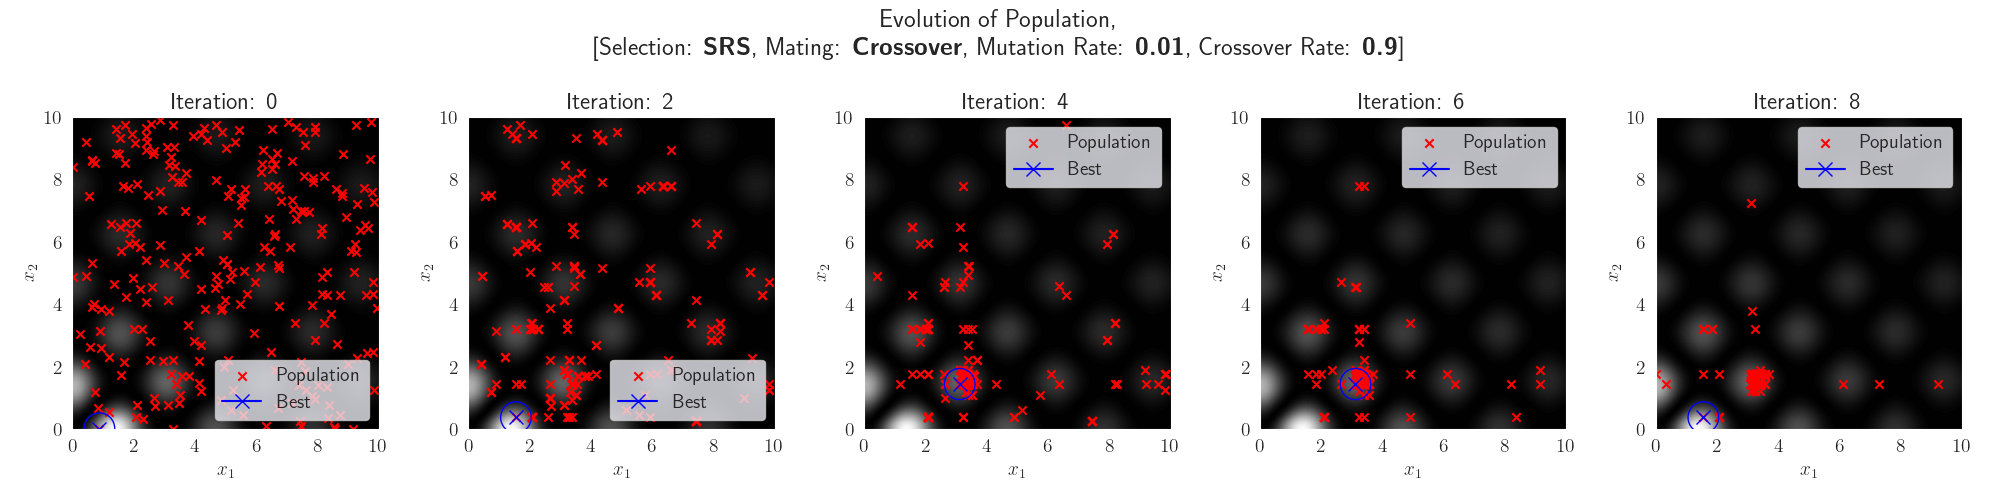
\includegraphics[width=\textwidth]{../figures/KBF/10_iters/SRS/Crossover/0.01_0.9_Population.png}
        \caption{Mutation Procedure: Crossover}
        \label{fig:CGA_flowchart_srs_crossover}
    \end{subfigure}
    \begin{subfigure}{\textwidth}
        \centering
        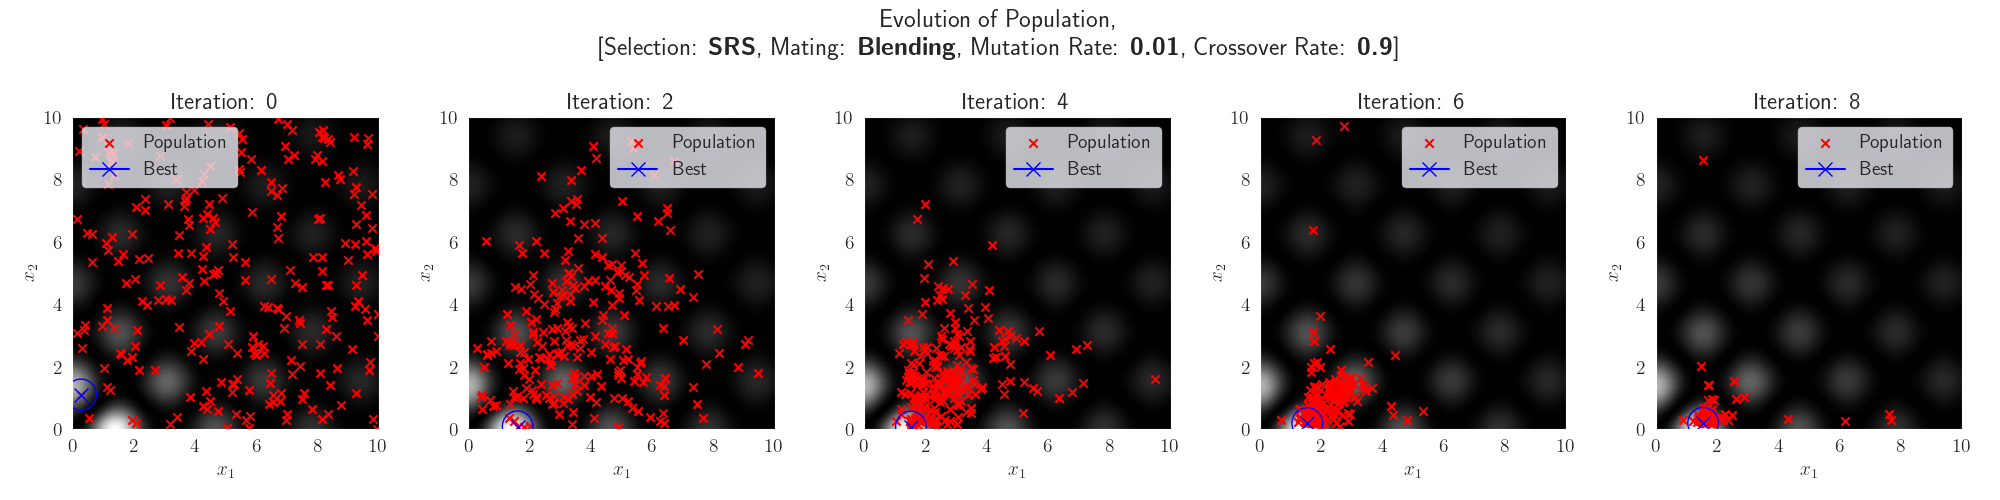
\includegraphics[width=\textwidth]{../figures/KBF/10_iters/SRS/Blending/0.01_0.9_Population.png}
        \caption{Mutation Procedure: Blending}
        \label{fig:CGA_flowchart_srs_blending}
    \end{subfigure}
    \captionsetup{justification=centering}
    \caption{Evolution of the population over 10 iterations using Stochastic Remainder Selection without Replacement (SRS). SRS was found to be the most effective selection method, when compared to Proportional Selection and Tournament Selection, as seen in Figures \ref{fig:CGA_flowchart_proportional} and \ref{fig:CGA_flowchart_tournament}, respectively.}
    \label{fig:CGA_flowchart_srs}
\end{figure}


\section{Methodology}
\section{Results}
\section{Discussion}
\section{Conclusion}
\bibliographystyle{plain}
\bibliography{refs} % Entries are in the refs.bib file

\section{Appendix}
\subsection{Supplementary Figures}
\begin{figure}[H]
    \centering
    \begin{subfigure}{\textwidth}
        \centering
        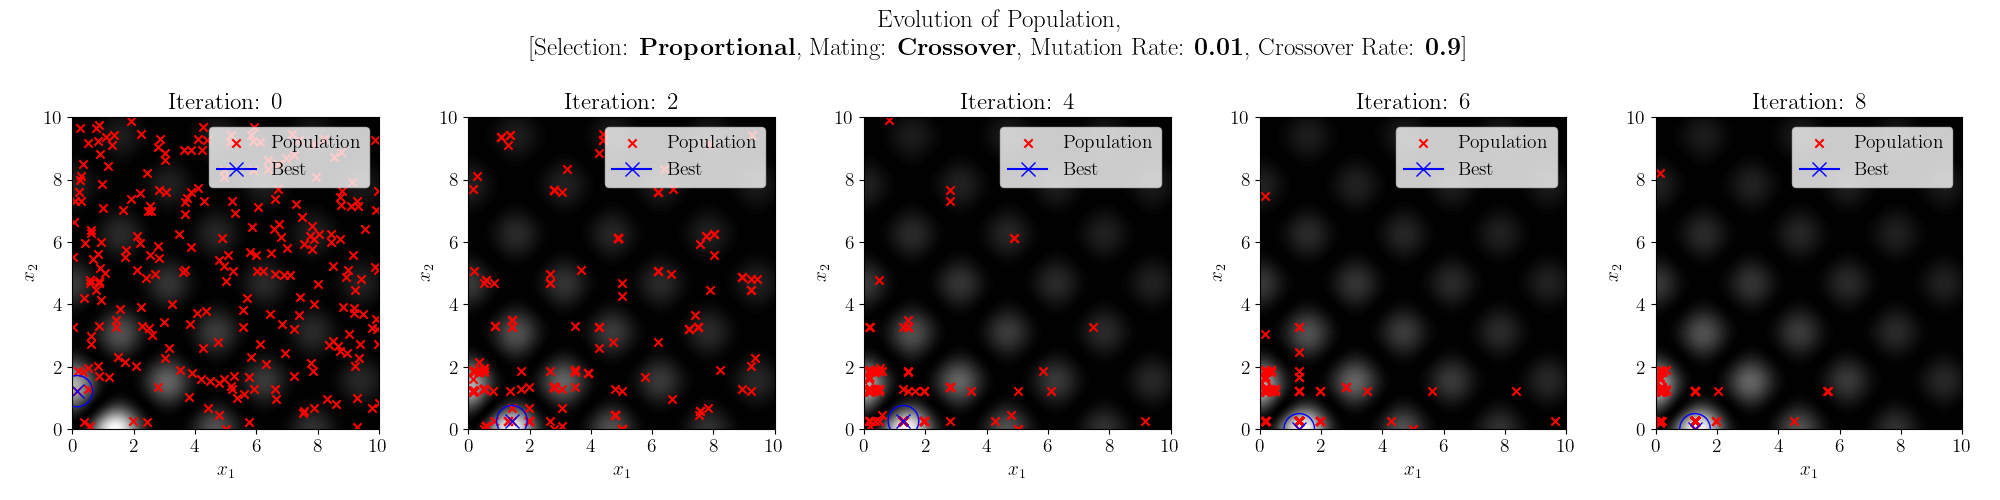
\includegraphics[width=\textwidth]{../figures/KBF/10_iters/Proportional/Crossover/0.01_0.9_Population.png}
        \caption{Mutation Procedure: Crossover}
        \label{fig:CGA_flowchart_proportional_crossover}
    \end{subfigure}
    \begin{subfigure}{\textwidth}
        \centering
        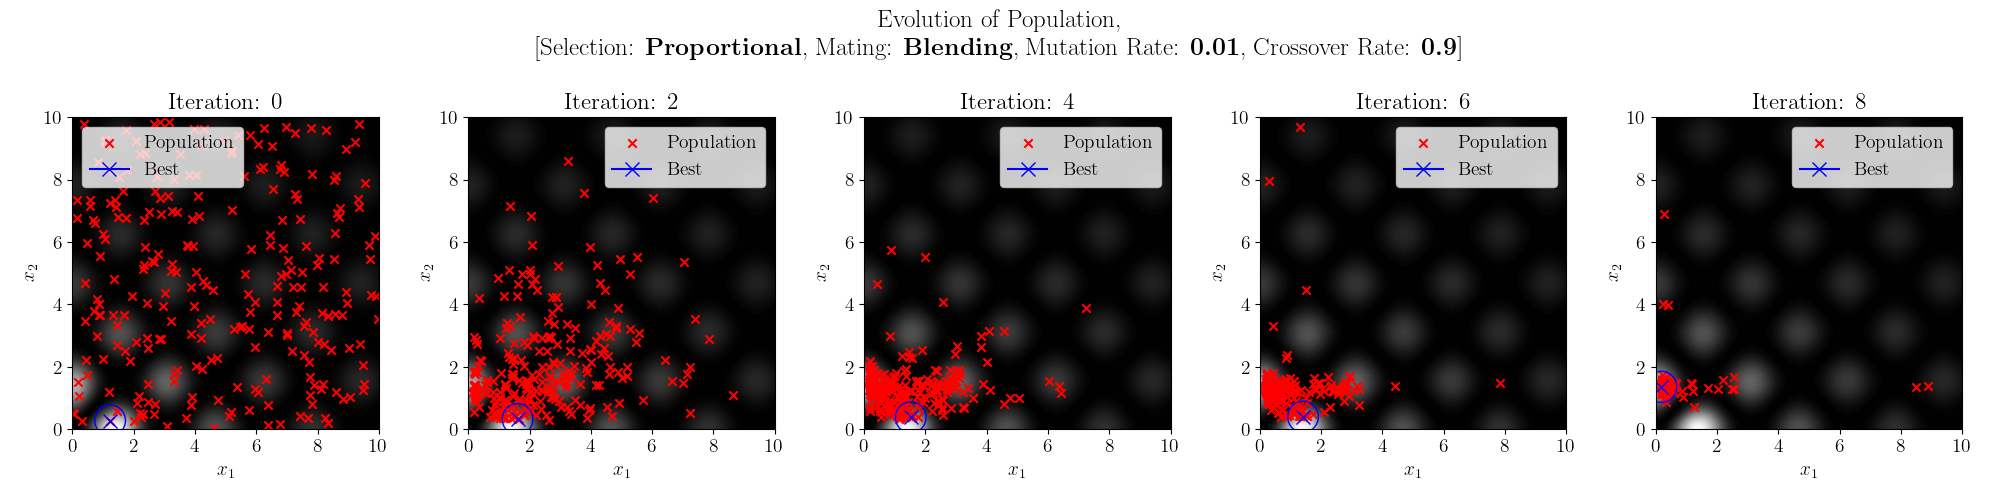
\includegraphics[width=\textwidth]{../figures/KBF/10_iters/Proportional/Blending/0.01_0.9_Population.png}
        \caption{Mutation Procedure: Blending}
        \label{fig:CGA_flowchart_proportional_blending}
    \end{subfigure}
    \captionsetup{justification=centering}
    \caption{Evolution of the population over 10 iterations using proportional selection. Proportional selection proved to be an effective selection method. However, it produced a larger final fitness value than SRS, and was therefore not chosen as the primary selection method.}
    \label{fig:CGA_flowchart_proportional}
\end{figure}

\begin{figure}[H]
    \centering
    \begin{subfigure}{\textwidth}
        \centering
        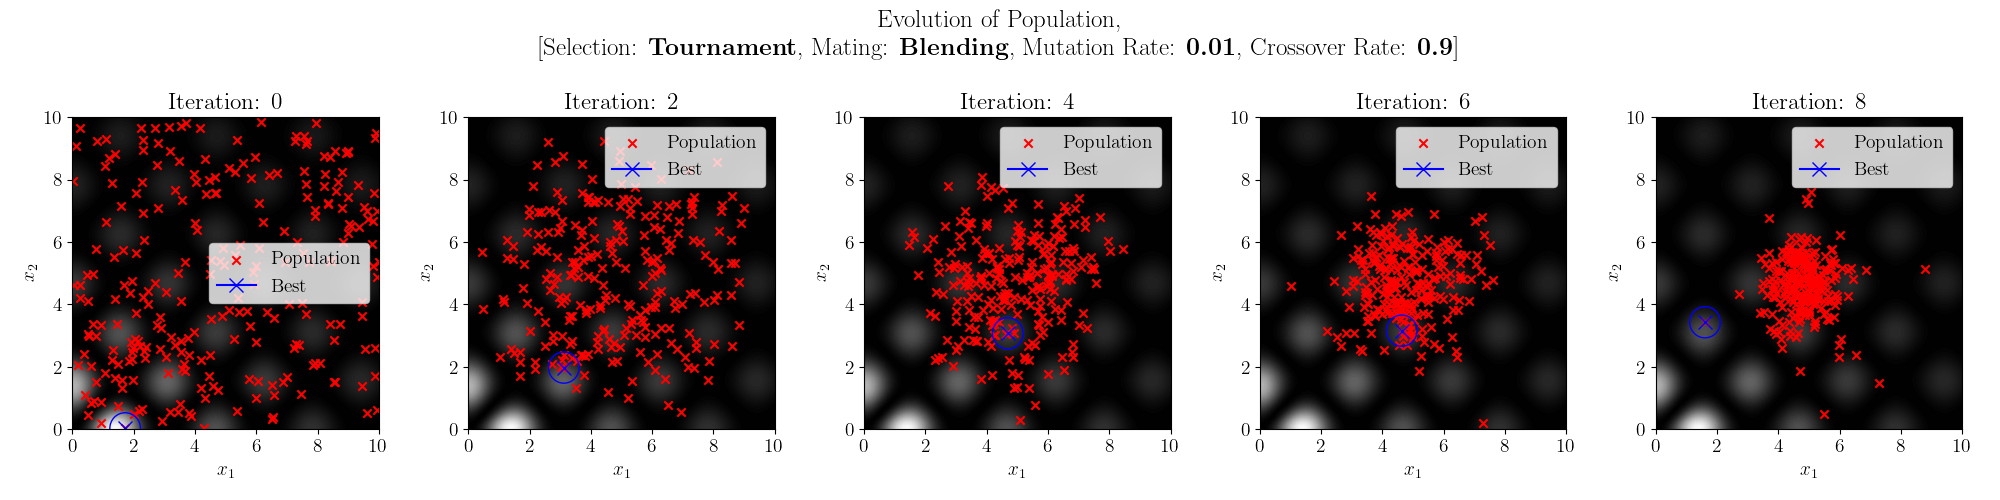
\includegraphics[width=\textwidth]{../figures/KBF/10_iters/Tournament/Blending/0.01_0.9_Population.png}
        \caption{Mutation Procedure: Blending}
        \label{fig:CGA_flowchart_tournament_blending}
    \end{subfigure}
    \begin{subfigure}{\textwidth}
        \centering
        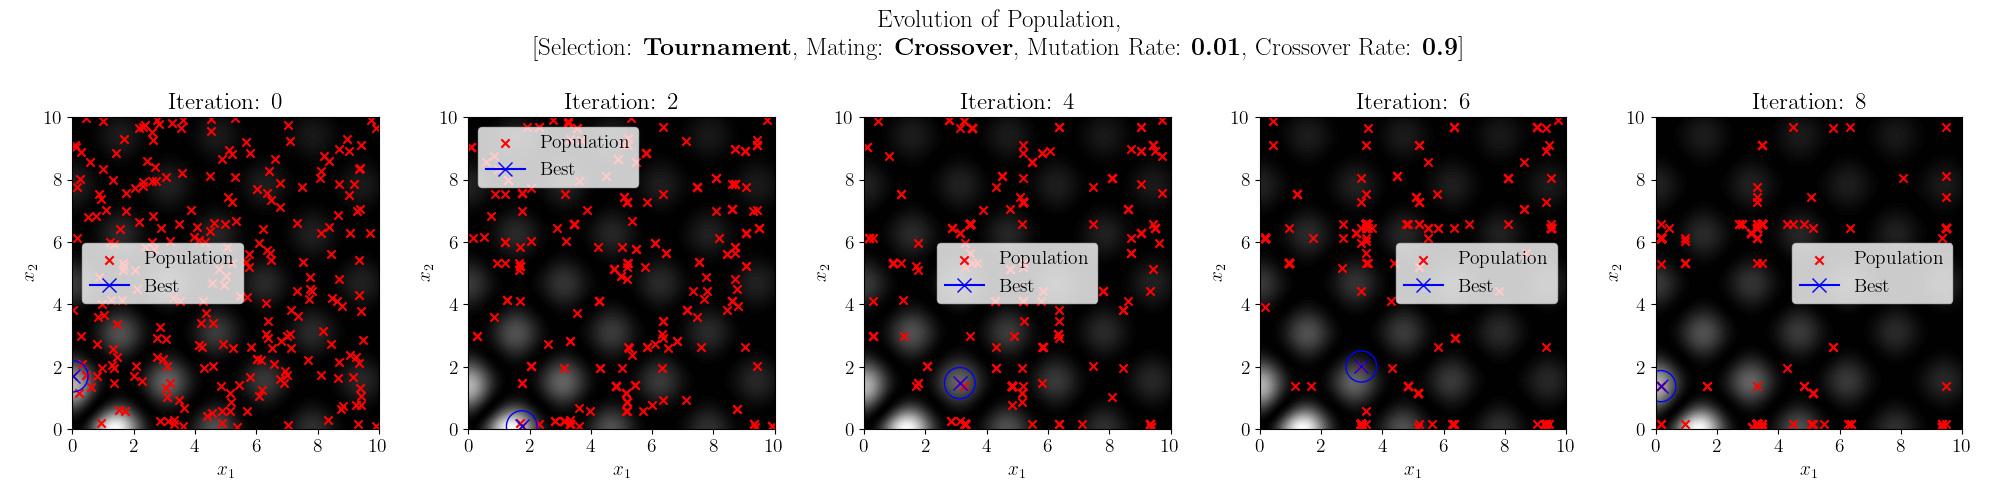
\includegraphics[width=\textwidth]{../figures/KBF/10_iters/Tournament/Crossover/0.01_0.9_Population.png}
        \caption{Mutation Procedure: Crossover}
        \label{fig:CGA_flowchart_tournament_crossover}
    \end{subfigure}
    \captionsetup{justification=centering}
    \caption{Evolution of the population over 10 iterations using Tournament Selection. Using Tournament Selection, the algorithm was unable to converge to a solution. Even 100 iterations produced a suboptimal solution, showcasing convergences to local optima, rather than the global optimum. As such, it was disregarded as a viable selection method.}
    \label{fig:CGA_flowchart_tournament}
\end{figure}

\end{document}